\section{Nastavování pájecích profilů pro BGA a QFN komponenty}
-termodesky, vztah teplotního profilu k parametrům DPS a pájecím slitinám, specifika pro různé způsoby ohřevu

\subsection{Termodesky}
Nevím, co se tím myslí. Snad to, že při pájení BGA, QFN je výhodnější použít i spodní ohřev, který nahřeje DPS a dojde tak k lepšímu a rychlejšímu přetavení při pájení (viz. Lab. úloha č. 4(BGA) v MPC-MTE).

\subsection{Vztah teplotního profilu k parametrům DPS a pájecím slitinám}
Nastavený teplotní profil musí respektovat typickou teplotu udávanou jako vrcholovou
teplotu pro aplikovaný typ pájecí slitiny superponovanou na výrobcem doporučovaný teplotní
profil použitého tavidla, nebo přímo výrobcem doporučovaný teplotní profil pájecí pasty. Dále
je potřeba zohlednit maximální doporučované teplotní odolnosti zpracovávaných součástek
a DPS.

U profilu \textbf{RTS} se vyskytuje méně problémů s pájitelností, nosič
tavidla vydrží déle v předehřívacím cyklu, což vede k lepšímu smáčení. Během lineárního
nárůstu dojde k předehřátí, k aktivaci tavidla, odpaření těkavých složek a minimalizaci teplotního šoku. Implementace RTS profilu snižuje energetické náklady, zvyšuje účinnost, redukuje pájecí defekty, zlepšuje smáčení i všeobecně zjednodušuje pájecí profil.

\begin{figure}[h]
   \begin{center}
     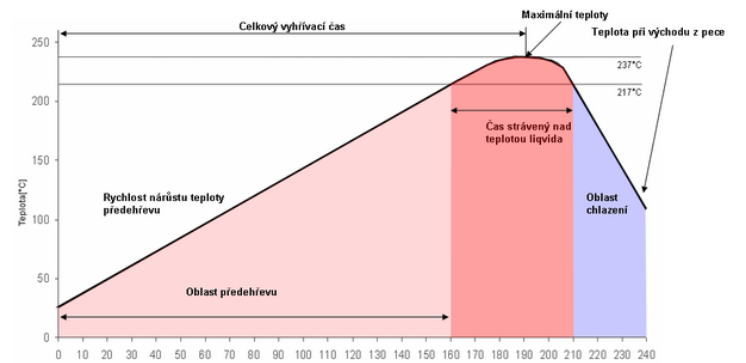
\includegraphics[scale=0.6]{images/RTS.png}
   \end{center}
   \caption{Ramp To Spike}
\end{figure}

\begin{figure}[h]
   \begin{center}
     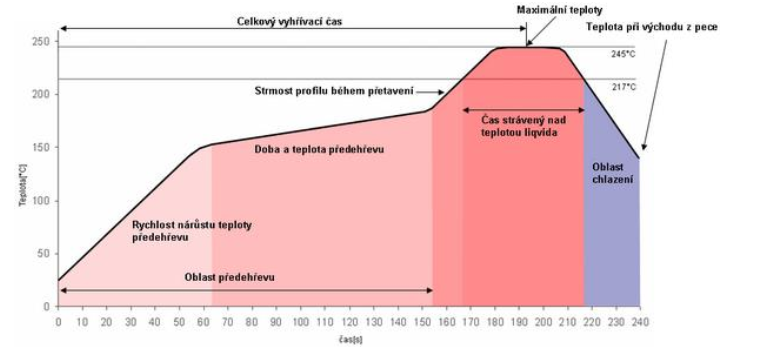
\includegraphics[scale=0.6]{images/RSS.png}
   \end{center}
   \caption{Ramp Soak Spike}
\end{figure}

\pagebreak
\subsection{Specifika pro různé způsoby ohřevu}

\subsubsection{Ohřev horkým vzduchem}
Pracují na poměrně jednoduchém principu - ofukování součástky horkým vzduchem ze speciálních trysek. Ty se liší svým tvarem a velikostí podle jednotlivých druhů součástek, pro které jsou určeny. Předností tohoto řešení je především jeho nízká cena a celkem dobrá univerzálnost. Dá se říci, že „kopíruje“ konvekční přetavovací pece, které pracují na stejném principu. Avšak zatímco ve velkých pecích je horký vzduch (v kombinaci s inertním plynem) takřka ideální kombinací, u malých stanic tomu tak není. Pec tvoří uzavřený homogenní systém, ve kterém se dají pouzdra BGA spolu s ostatními součástkami spolehlivě zapájet. Opravárenská stanice není uzavřeným systémem. Tryska není nikdy zcela bez otvorů, anebo nedosedá až na povrch DPS - vzduch musí někudy
proudit ven. A právě to je příčinou některých problémů:
\begin{itemize}
\item Horký vzduch ofukuje i okolní součástky - hrozí jejich natavení a jsou-li malé, tak i jejich odfouknutí. Je třeba je chránit kaptonovou páskou nebo krycí fólií, což zvyšuje spotřebu materiálu a prodlužuje pájecí proces. Lepidlo z pásky navíc znečišťuje DPS  a nechává po sobě stopy.
\item  Vzduch v trysce kvůli svému turbulentnímu proudění neohřívá součástku (hlavně větší BGA pouzdra) rovnoměrně.
\item  Pokud tryska dosedá až na povrch DPS, neumožňuje optickou kontrolu průběhu pájecího procesu (dvojí pokles).
\item  Úspěšné zapájení součástky je silně závislé na mnoha vzájemně provázaných
parametrech - tlak vzduchu, teplota, čas, tvar trysky a její přiblížení k součástce
\end{itemize}
Tyto stanice navíc vyžadují externí přívod stlačeného vzduchu, což omezuje rozsah jejich
použití a zvyšuje náklady na instalaci (vzduchové rozvody, kompresor, atd).

\subsubsection{IR ohřev}
Využívají k ohřevu součástek IR záření ze speciálních zářičů.
Nejedná se o viditelné tepelné záření, které je možné vidět u většiny spodních předehřevů, ale často o úzkopásmové středovlnné IR záření ($\lambda$ = 2-8 $\mu$m). Záření této vlnové délky má prokazatelně nejlepší poměr absorpce/reflexe v prostředí viditelného i neviditelného spektra. Proto je jeho účinnost téměř nezávislá na materiálu a barvě pouzdra součástky. Od toho se
odvíjí i řada následujících výhod:
\begin{itemize}
\item Plocha součástky je rovnoměrně ohřívána a nehrozí její poškození
v důsledku přehřátí.
\item Okolní součástky nejsou nijak ovlivňovány - efektivní plocha zářičů se dá upravit
nastavitelnými stínícími lamelami tak, že záření působí jen na ploše pájeného pouzdra.
\item Zářiče jsou od součástky dostatečně vzdáleny, takže je možné snadno opticky
kontrolovat průběh pájecího procesu.
\item Počet nastavovaných parametrů je menší - v podstatě jen teplota a čas.
\end{itemize}
V porovnání s horkovzdušnými systémy navíc odpadají nákladné rozvody stlačeného
vzduchu. Nevýhodou IR systémů je vyšší pořizovací cena.


